\documentclass[tikz, border=14pt]{standalone}
\usepackage{circuitikz}
\usepackage{amsmath}

% ============================================================
%  EPE2316 – 3-Bus Power System Diagram  (v2 – correct bus taps)
%
%  KEY CONVENTION: conductors approach bus bars at 90 degrees.
%  Each transmission line taps the bus bar at a distinct point,
%  making T-junctions clearly visible. Short orthogonal stubs
%  connect the diagonal runs to the bars.
%
%  Bus 1 (Slack) : vertical bar at x=1.5
%  Bus 2 (PQ)    : vertical bar at x=9.0
%  Bus 3 (PV)    : horizontal bar at y=5.5, x=4.5 to 6.0
%
%  Line routing:
%   L1-2 : horizontal, y=0, from Bus1 to Bus2 (no elbow needed)
%   L1-3 : tap Bus1 at (1.5, 0.35) -> short horizontal stub left
%           -> diagonal up-right -> short horizontal stub right
%           -> tap Bus3 at (4.5, 5.5)
%   L2-3 : tap Bus2 at (9.0, 0.35) -> short horizontal stub right
%           -> diagonal up-left -> short horizontal stub left
%           -> tap Bus3 at (6.0, 5.5)
%
%  System base: S_base = 100 MW,  V_base = 22 kV
% ============================================================

\begin{document}
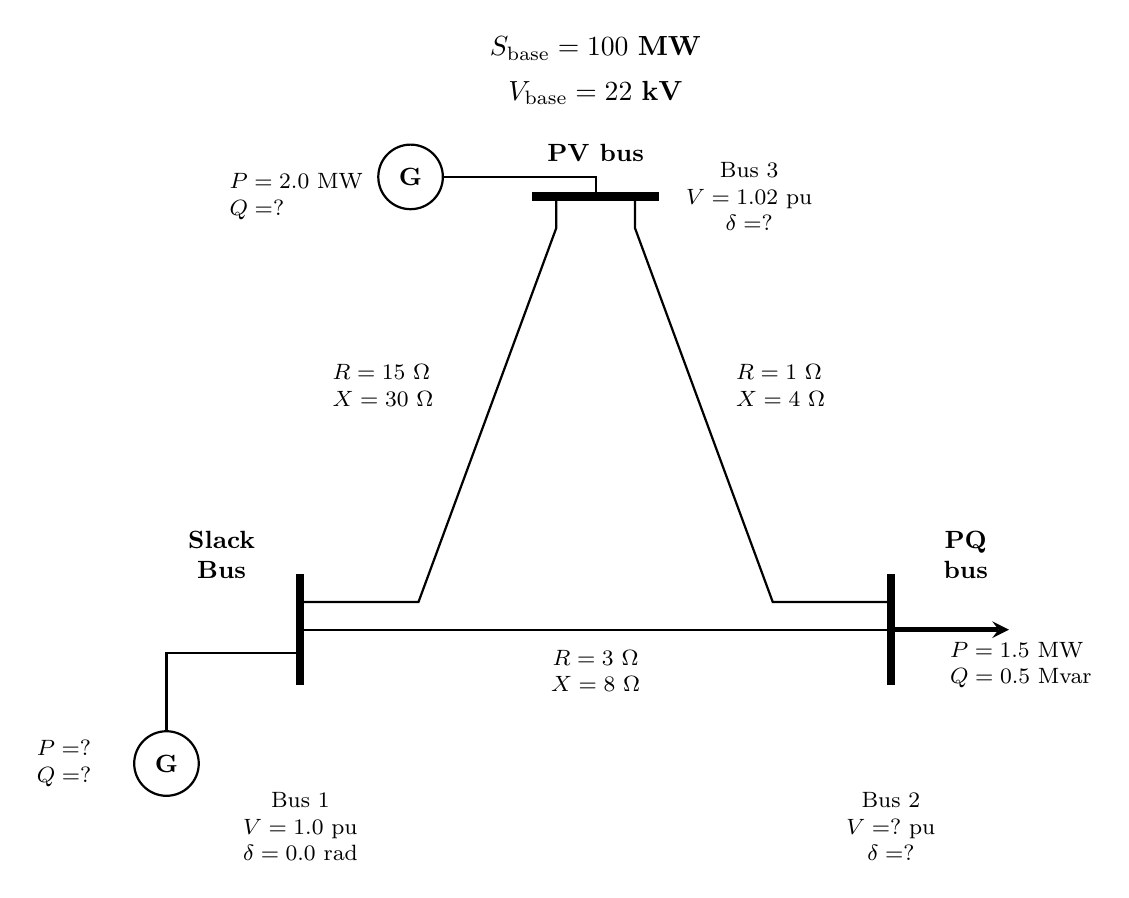
\begin{tikzpicture}[
    bus/.style       = {line width=3pt, line cap=rect},
    conductor/.style = {thick},
    genbox/.style    = {circle, draw, thick, minimum size=0.82cm,
                        inner sep=0pt, font=\small\bfseries},
    loadarrow/.style = {->, >=stealth, line width=1.6pt},
    lbl/.style       = {font=\small\bfseries, align=center},
    ann/.style       = {font=\footnotesize, align=center},
    param/.style     = {font=\footnotesize, align=left},
]

% ============================================================
%  BUS 1  –  Slack Bus (bottom-left), vertical bar at x=1.5
% ============================================================
\draw[bus] (1.5, -0.65) -- (1.5, 0.65);

% Generator: elbow left then down from lower tap
\node[genbox] (G1) at (-0.2, -1.7) {G};
\draw[conductor] (1.5, -0.3) -- (-0.2, -0.3) -- (G1.north);
\node[param] at (-1.5, -1.7) {$P = ?$\\$Q = ?$};
\node[lbl]   at (0.5, 0.95)  {Slack\\Bus};
\node[ann]   at (1.5, -2.5)
    {Bus 1\\$V = 1.0\ \mathrm{pu}$\\$\delta = 0.0\ \mathrm{rad}$};

% ============================================================
%  BUS 2  –  PQ Bus (bottom-right), vertical bar at x=9.0
% ============================================================
\draw[bus] (9.0, -0.65) -- (9.0, 0.65);

\draw[loadarrow] (9.0, 0) -- (10.5, 0);
\node[param] at (10.65, -0.45) {$P = 1.5\ \mathrm{MW}$\\$Q = 0.5\ \mathrm{Mvar}$};
\node[lbl]   at (9.95, 0.95) {PQ\\bus};
\node[ann]   at (9.0, -2.5)
    {Bus 2\\$V = ?\ \mathrm{pu}$\\$\delta = ?$};

% ============================================================
%  BUS 3  –  PV Bus (top-centre), horizontal bar at y=5.5
% ============================================================
\draw[bus] (4.5, 5.5) -- (6.0, 5.5);

\node[genbox] (G3) at (2.9, 5.75) {G};
\draw[conductor] (G3.east) -- (5.25, 5.75) -- (5.25, 5.5);
\node[param] at (1.45, 5.5)  {$P = 2.0\ \mathrm{MW}$\\$Q = ?$};
\node[lbl]   at (5.25, 6.05) {PV bus};
\node[ann]   at (7.2, 5.5)
    {Bus 3\\$V = 1.02\ \mathrm{pu}$\\$\delta = ?$};

% ============================================================
%  TRANSMISSION LINE 1–2   R = 3 Ohm,  X = 8 Ohm
%  Pure horizontal run – both bus bars are at y=0, no elbow needed.
%  Taps Bus 1 at (1.5, 0) and Bus 2 at (9.0, 0).
% ============================================================
\draw[conductor] (1.5, 0) -- (9.0, 0);
\node[ann] at (5.25, -0.52) {$R = 3\ \Omega$\\$X = 8\ \Omega$};

% ============================================================
%  TRANSMISSION LINE 1–3   R = 15 Ohm,  X = 30 Ohm
%
%  Three segments – forms an angled run but with 90-deg stubs
%  at both bus bar ends so the tap is always perpendicular:
%
%    (1.5,  0.35)  upper tap on Bus 1 vertical bar
%    (1.0,  0.35)  short horizontal stub LEFT  (clears the bar)
%    (4.5,  5.2 )  diagonal run up-right
%    (4.5,  5.5 )  short vertical stub UP into Bus 3
% ============================================================
\draw[conductor]
    (1.5,  0.35)   % tap on Bus 1 (upper)
    -- (3.0,  0.35)   % stub: move left so diagonal clears bar
    -- (4.75,  5.1)    % diagonal up to just below Bus 3
    -- (4.75,  5.5);   % stub: vertical into Bus 3 tap

\node[param] at (2.55, 3.1) {$R = 15\ \Omega$\\$X = 30\ \Omega$};

% ============================================================
%  TRANSMISSION LINE 2–3   R = 1 Ohm,  X = 4 Ohm
%
%    (9.0,  0.35)  upper tap on Bus 2 vertical bar
%    (9.5,  0.35)  short horizontal stub RIGHT (clears the bar)
%    (6.0,  5.2 )  diagonal run up-left
%    (6.0,  5.5 )  short vertical stub UP into Bus 3
% ============================================================
\draw[conductor]
    (9.0,  0.35)   % tap on Bus 2 (upper)
    -- (7.5,  0.35)   % stub: move right so diagonal clears bar
    -- (5.75,  5.1)    % diagonal up-left to just below Bus 3
    -- (5.75,  5.5);   % stub: vertical into Bus 3 tap

\node[param] at (7.6, 3.1) {$R = 1\ \Omega$\\$X = 4\ \Omega$};

% ============================================================
%  TITLE  –  System base values
% ============================================================
\node[font=\normalsize, align=center] at (5.25, 7.1)
    {$S_{\text{base}} = 100\ \mathbf{MW}$\\[4pt]
     $V_{\text{base}} = 22\ \mathbf{kV}$};

\end{tikzpicture}
\end{document}
